\section*{Dictionnaire de données}

On identifie les données utiles au système d'information à partir du recueil informel des besoins.

\begin{figure}[!h]
\begin{tabular}{l l l l l l}
%
    \textbf{mnémonique} & \textbf{desc.} & \textbf{type} & \textbf{format} & \textbf{divers} & \textbf{exemple} \\
    id-ticket            & - & entier  & -          & séquentiel & 1 \\
    date-ticket          & - & date    & jj/mm/aaaa & -          & 01/01/2001 \\
    nb-personnes         & - & entier  & -          & -          & 3 \\
    no-fiche-de-paye     & - & entier  & -          & séquentiel & 1 \\
    date-début-période   & - & date    & jj/mm/aaaa & -          & 01/01/2001 \\
    date-fin-période     & - & date    & jj/mm/aaaa & -          & 01/01/2001 \\
    salaire              & - & décimal & -          & -          & 1532.30 \\
    no-employé           & - & entier  & -          & séquentiel & 1 \\
    nom-employé          & - & texte   & 50 car.    & -          & Arthur Hugo \\
    en-soirée            & - & booléen & -          & -          & Vrai \\
    date-venue           & - & date    & jj/mm/aaaa & -          & 01/01/2001 \\
%
\end{tabular}
    \caption{\label{DD} Dictionnaire de données}
\end{figure}

\newpage
\section*{Diagramme de Flux}

On identifie les flux d'information en fonction du recueil informel des besoins.

\begin{figure}[!htb]
    \begin{center}
    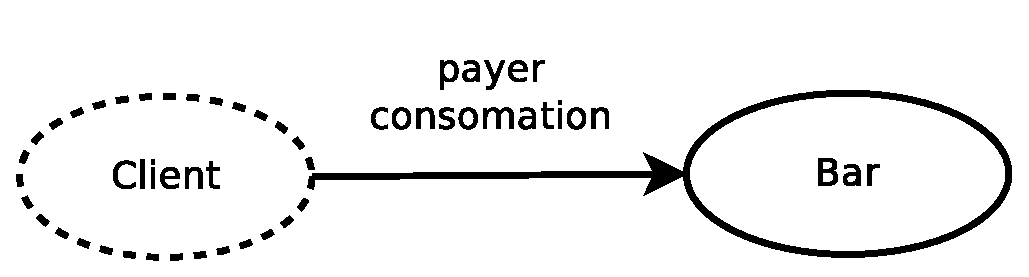
\includegraphics[width=6cm]{images/cc1_df1.eps}
    \caption{\label{cc1_df1} Diagramme de contexte}
    \end{center}
\end{figure}

\begin{figure}[!htb]
    \begin{center}
    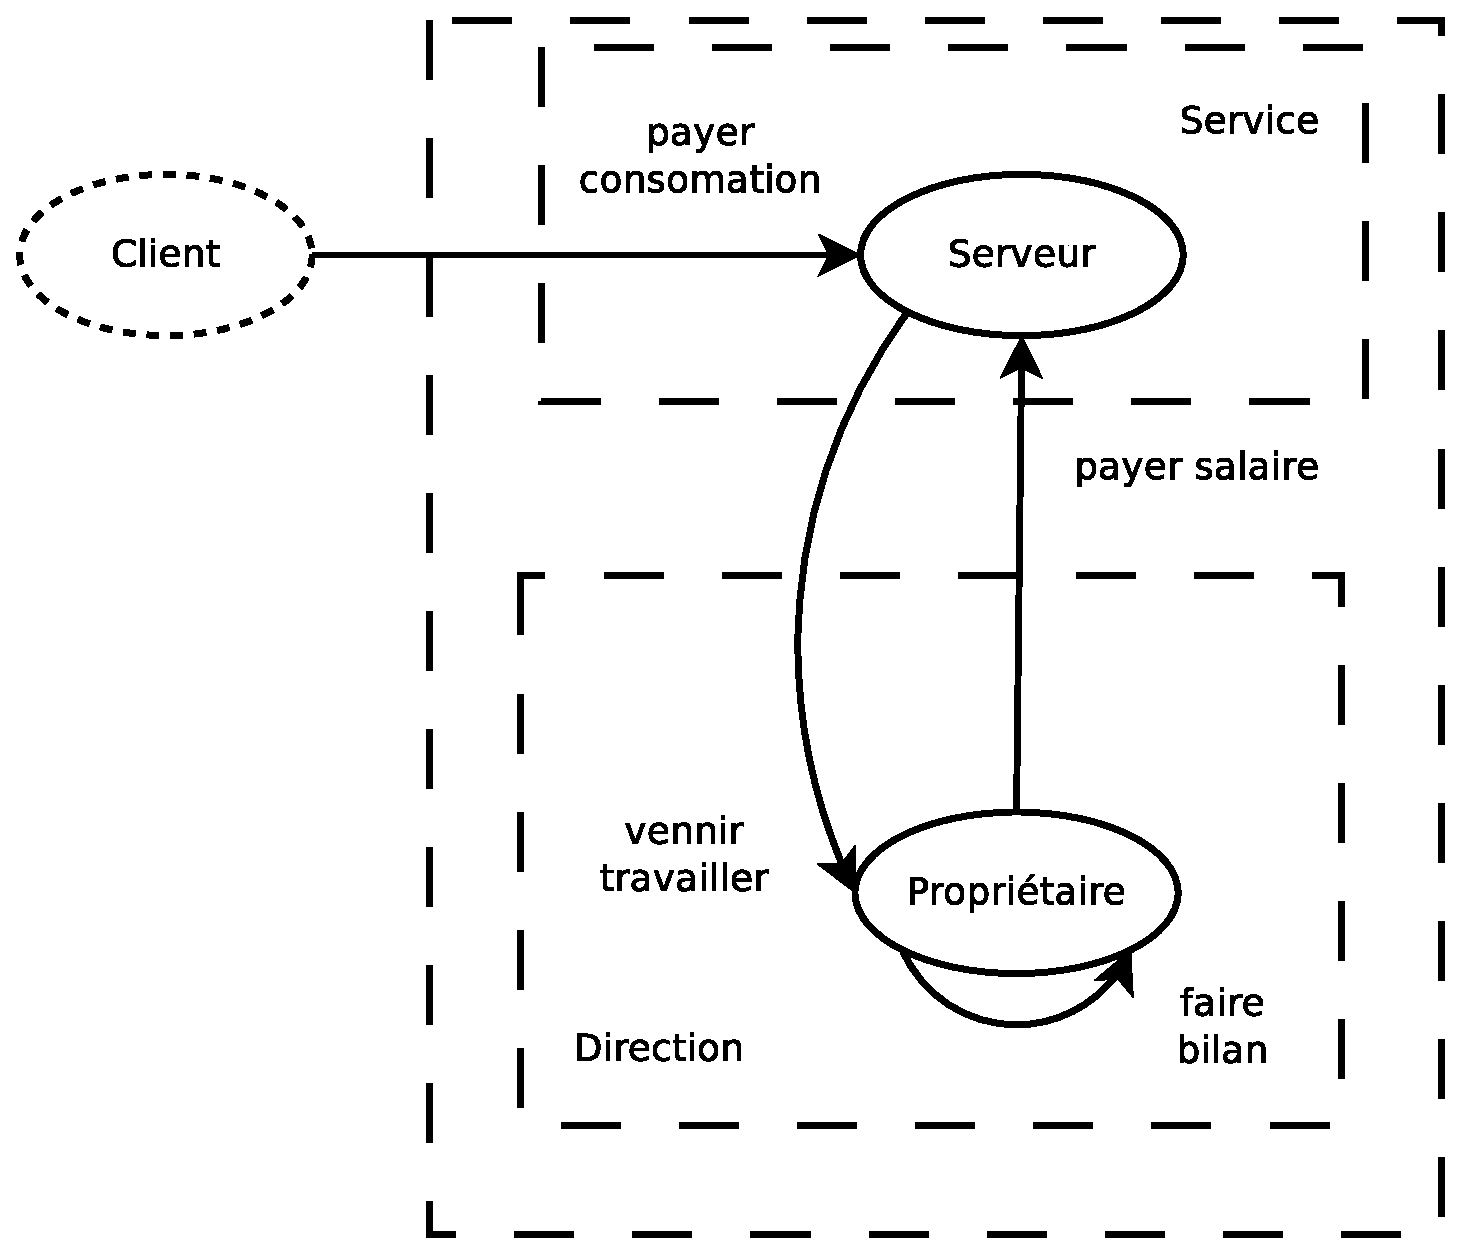
\includegraphics[width=9cm]{images/cc1_df2.eps}
    \caption{\label{cc1_df3} Diagramme de flux}
    \end{center}
\end{figure}

\section*{Matrice des Flux}

À faire à partir du diagramme de flux.

\newpage
\section*{Modèle Concptuel de Communication}

Pour chaque flux d'information du diagramme de flux, on détaille les messages échangés.

\begin{figure}[!htb]
    \begin{center}
    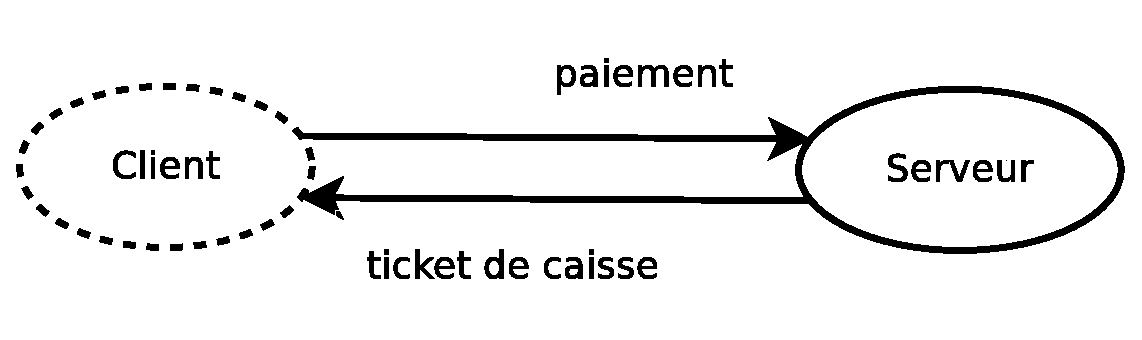
\includegraphics[width=6cm]{images/cc1_mcc1.eps}
    \caption{\label{cc1_mcc1} payer consomation}
    \end{center}
\end{figure}

\begin{figure}[!htb]
    \begin{center}
    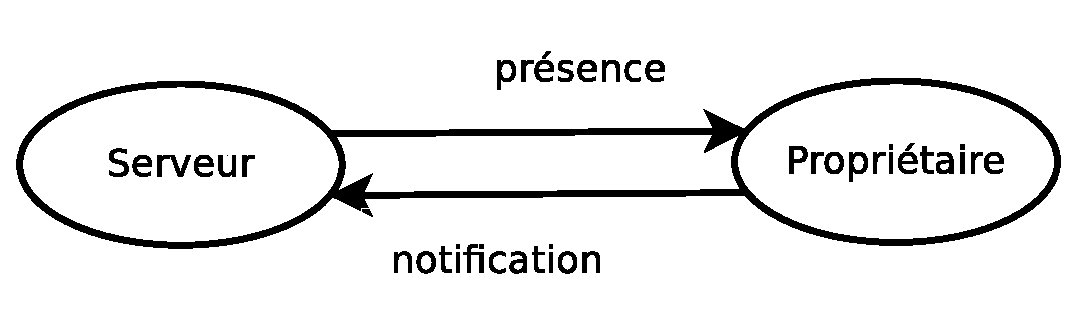
\includegraphics[width=6cm]{images/cc1_mcc2.eps}
    \caption{\label{cc1_mcc2} venir travailler}
    \end{center}
\end{figure}

\begin{figure}[!htb]
    \begin{center}
    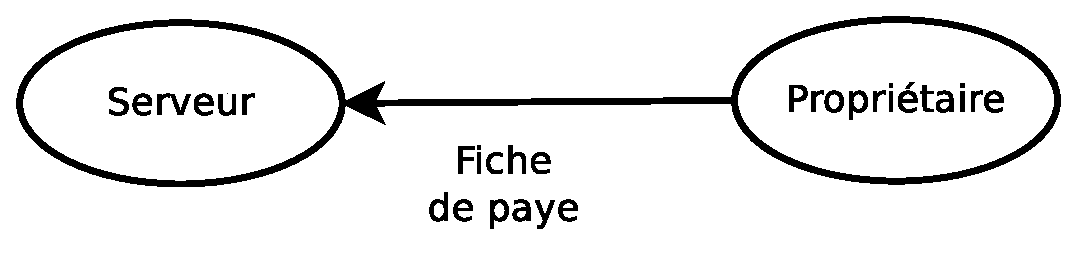
\includegraphics[width=6cm]{images/cc1_mcc3.eps}
    \caption{\label{cc1_mcc3} payer salaire}
    \end{center}
\end{figure}

\begin{figure}[!htb]
    \begin{center}
    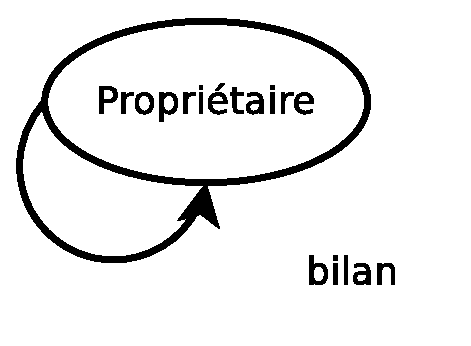
\includegraphics[width=3cm]{images/cc1_mcc4.eps}
    \caption{\label{cc1_mcc4} faire bilan}
    \end{center}
\end{figure}

\newpage
\section*{Modèle Concptuel de Communication détaillé}

On place affecte maintenant chaque donnée du dictionnaire de données dans le message qui la contient.

\subsubsection*{paiement (Client, Serveur)}
\begin{itemize}
    \item nb-personnes
\end{itemize}

\subsubsection*{ticket de caisse (Serveur, Client)}
\begin{itemize}
    \item date-ticket
    \item no-employé
\end{itemize}

\subsubsection*{présence (Serveur, Propriétaire)}
\begin{itemize}
    \item nom-employé
    \item date-venue
    \item en-soirée
\end{itemize}

\subsubsection*{notification (Propriétaire, Serveur)}
\begin{itemize}
    \item no-employé
    \item date-venue
    \item en-soirée
\end{itemize}

\subsubsection*{fiche de paye (Propriétaire, Serveur)}
\begin{itemize}
    \item no-fiche-de-paye
    \item date-salaire
    \item salaire
    \item prime*
    \item no-employé
    \item nom-employé
\end{itemize}

\subsubsection*{bilan (Propriétaire, Propriétaire)}
\begin{itemize}
    \item date-debut-période
    \item date-fin-période
    \item nb-clients-journée*
    \item nb-clients-soirée*
\end{itemize}

\newpage
\section*{Modèle Conceptuel de Données}

En suivant l'ordre des messages du MCC, on place chaque donnée véhiculée par un message dans le MCD. Pour chaque donnée, on se pose la question de l'existance d'une nouvelle entité. Une fois toutes les données placées, on valide notre MCD (formes normales).

\begin{figure}[!htb]
    \begin{center}
    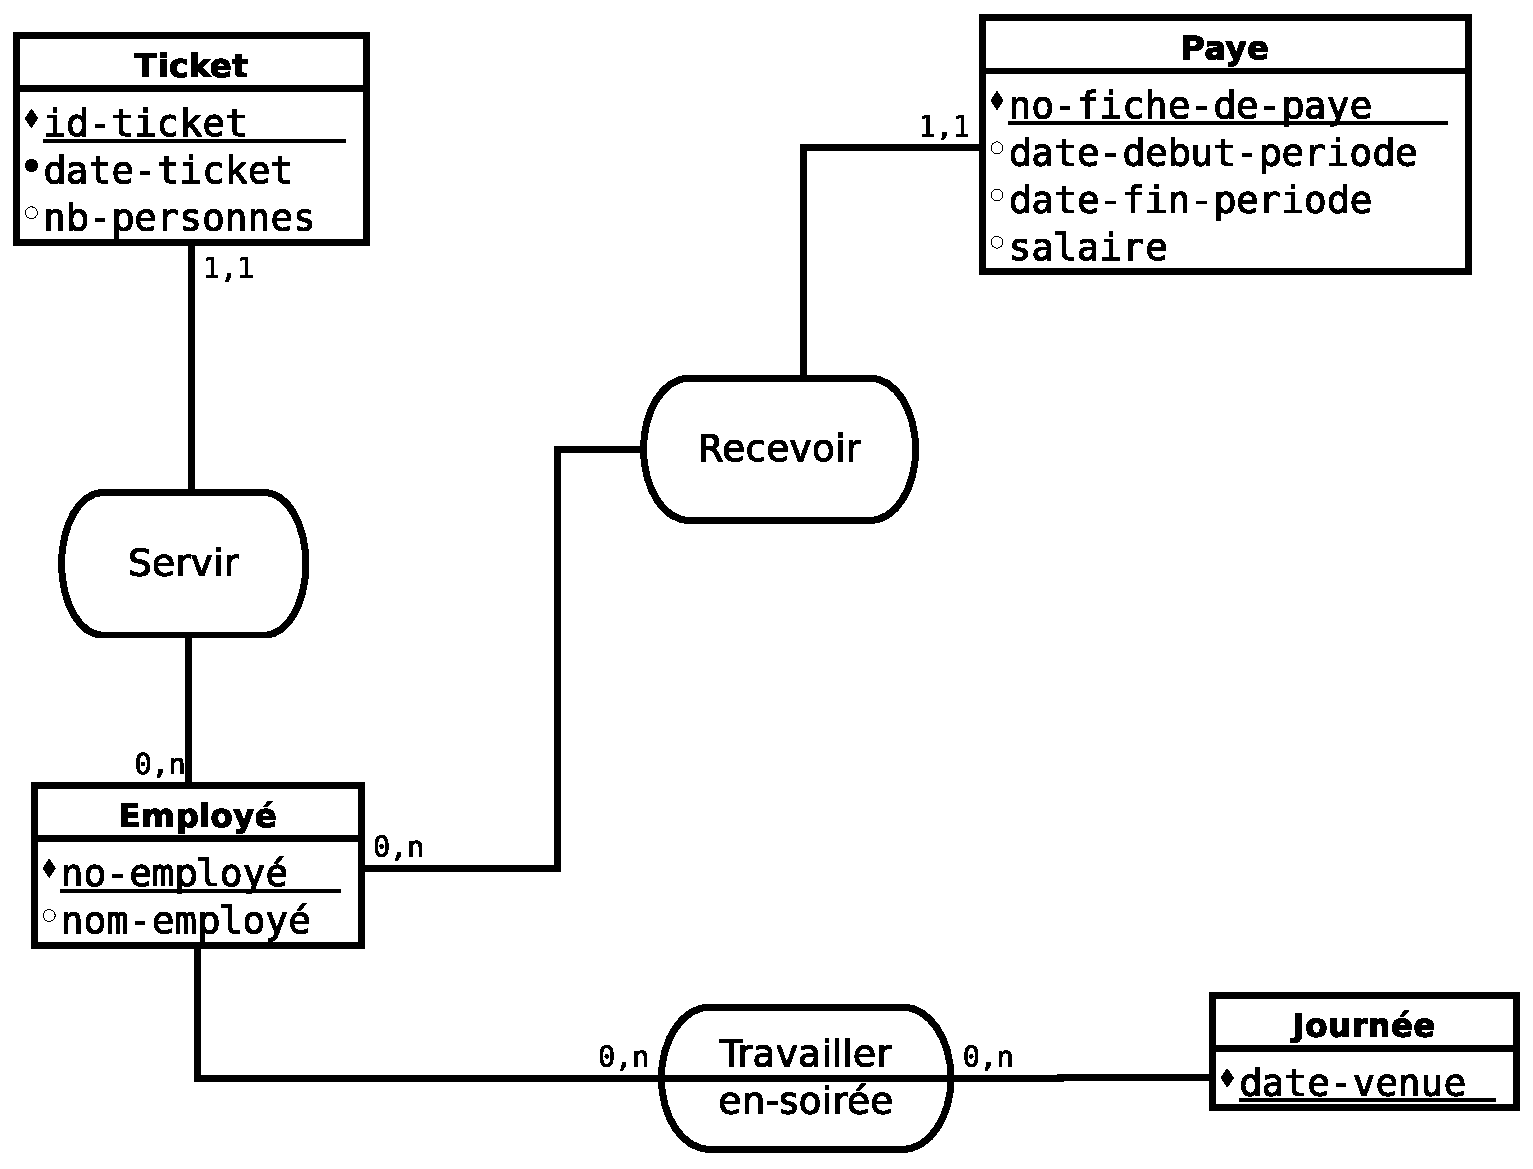
\includegraphics[width=11.5cm]{images/cc1_mcd.eps}
    \caption{\label{cc1_mcd} MCD}
    \end{center}
\end{figure}

\newpage
\section*{Modèle Conceptuel de Traitements}

Pour chaque acteur, on se demande les actions qu'il effectue sur notre système d'information.

\begin{figure}[!htb]
    \begin{center}
    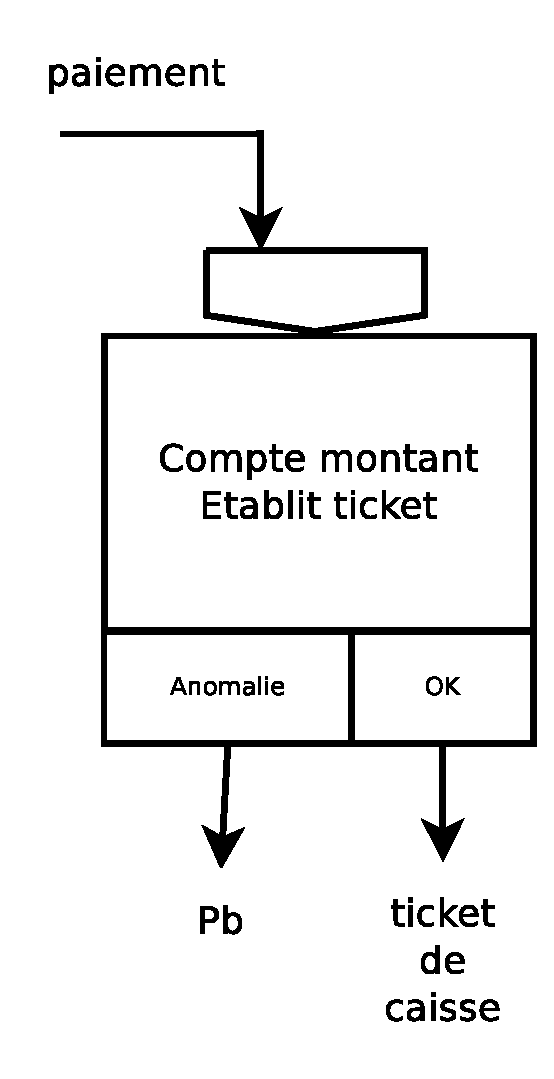
\includegraphics[height=7cm]{images/cc1_mct1.eps}
    \caption{\label{cc1_mct1} Servir une consomation}
    \end{center}
\end{figure}

\begin{figure}[!htb]
    \begin{center}
    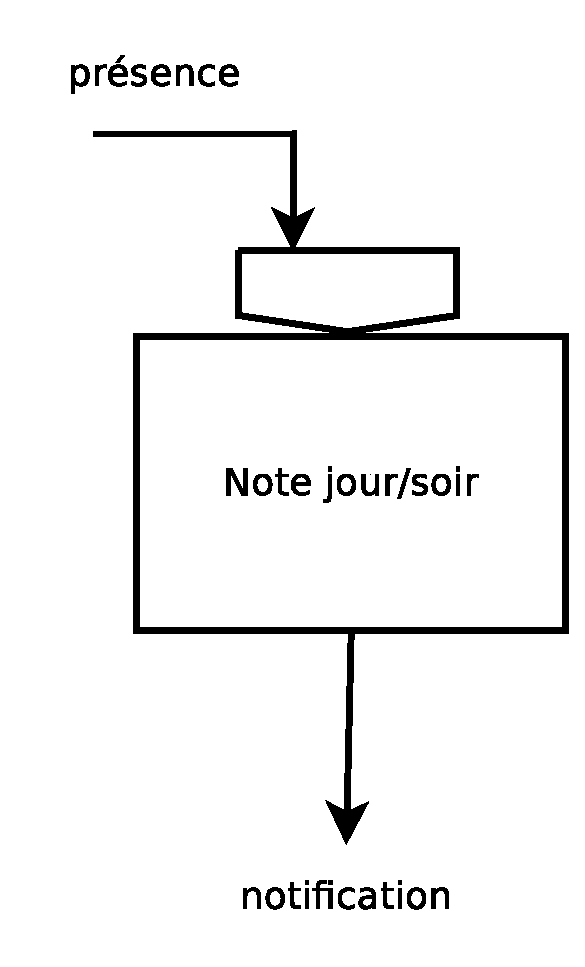
\includegraphics[height=7cm]{images/cc1_mct2.eps}
    \caption{\label{cc1_mct2} Venir travailler}
    \end{center}
\end{figure}

\begin{figure}[!htb]
    \begin{center}
    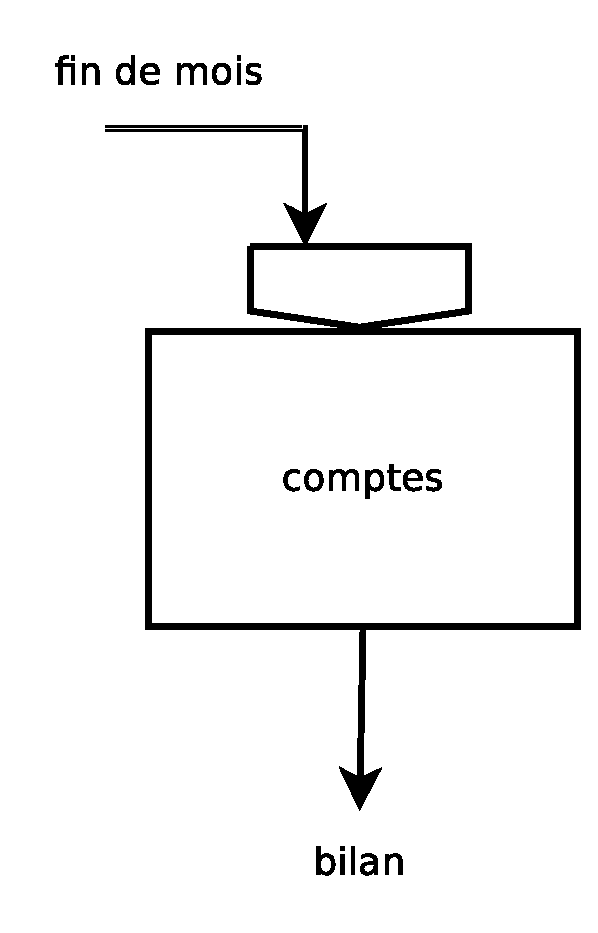
\includegraphics[height=7cm]{images/cc1_mct3.eps}
    \caption{\label{cc1_mct3} Faire un bilan}
    \end{center}
\end{figure}

\begin{figure}[!htb]
    \begin{center}
    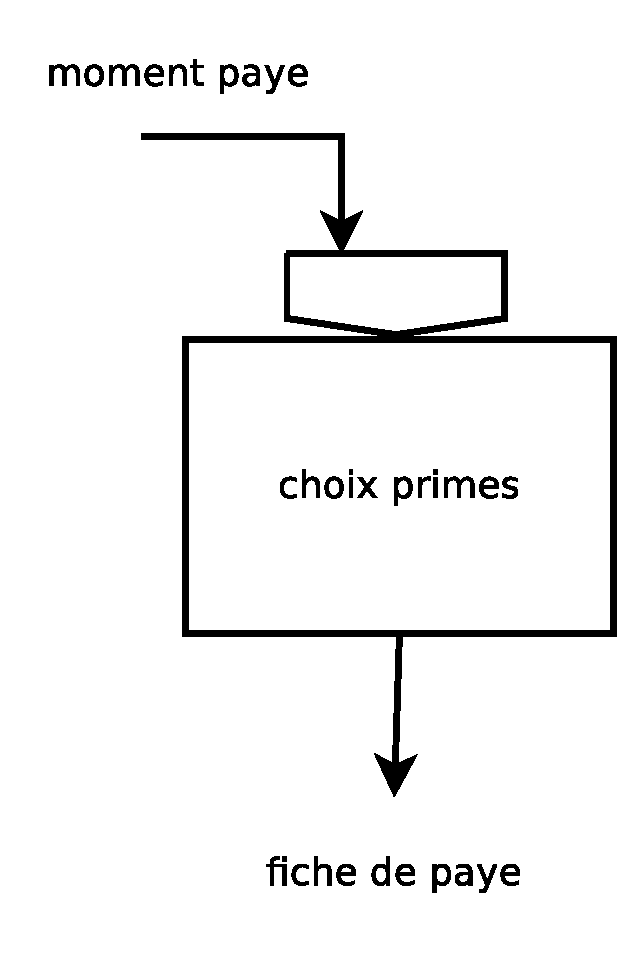
\includegraphics[height=7cm]{images/cc1_mct4.eps}
    \caption{\label{cc1_mct4} Calculer un salaire}
    \end{center}
\end{figure}

\newpage
\section*{Modèle Organisationel de Traitements}

On commence par déterminer les différents postes de travail d'utilisation de notre système d'information :\\

\begin{itemize}
    \item
    %\item Bureau du club
    %\item Bureau des homologation
    %\item Bureau de classement
\end{itemize}

\begin{figure}[!htb]
    \begin{center}
    %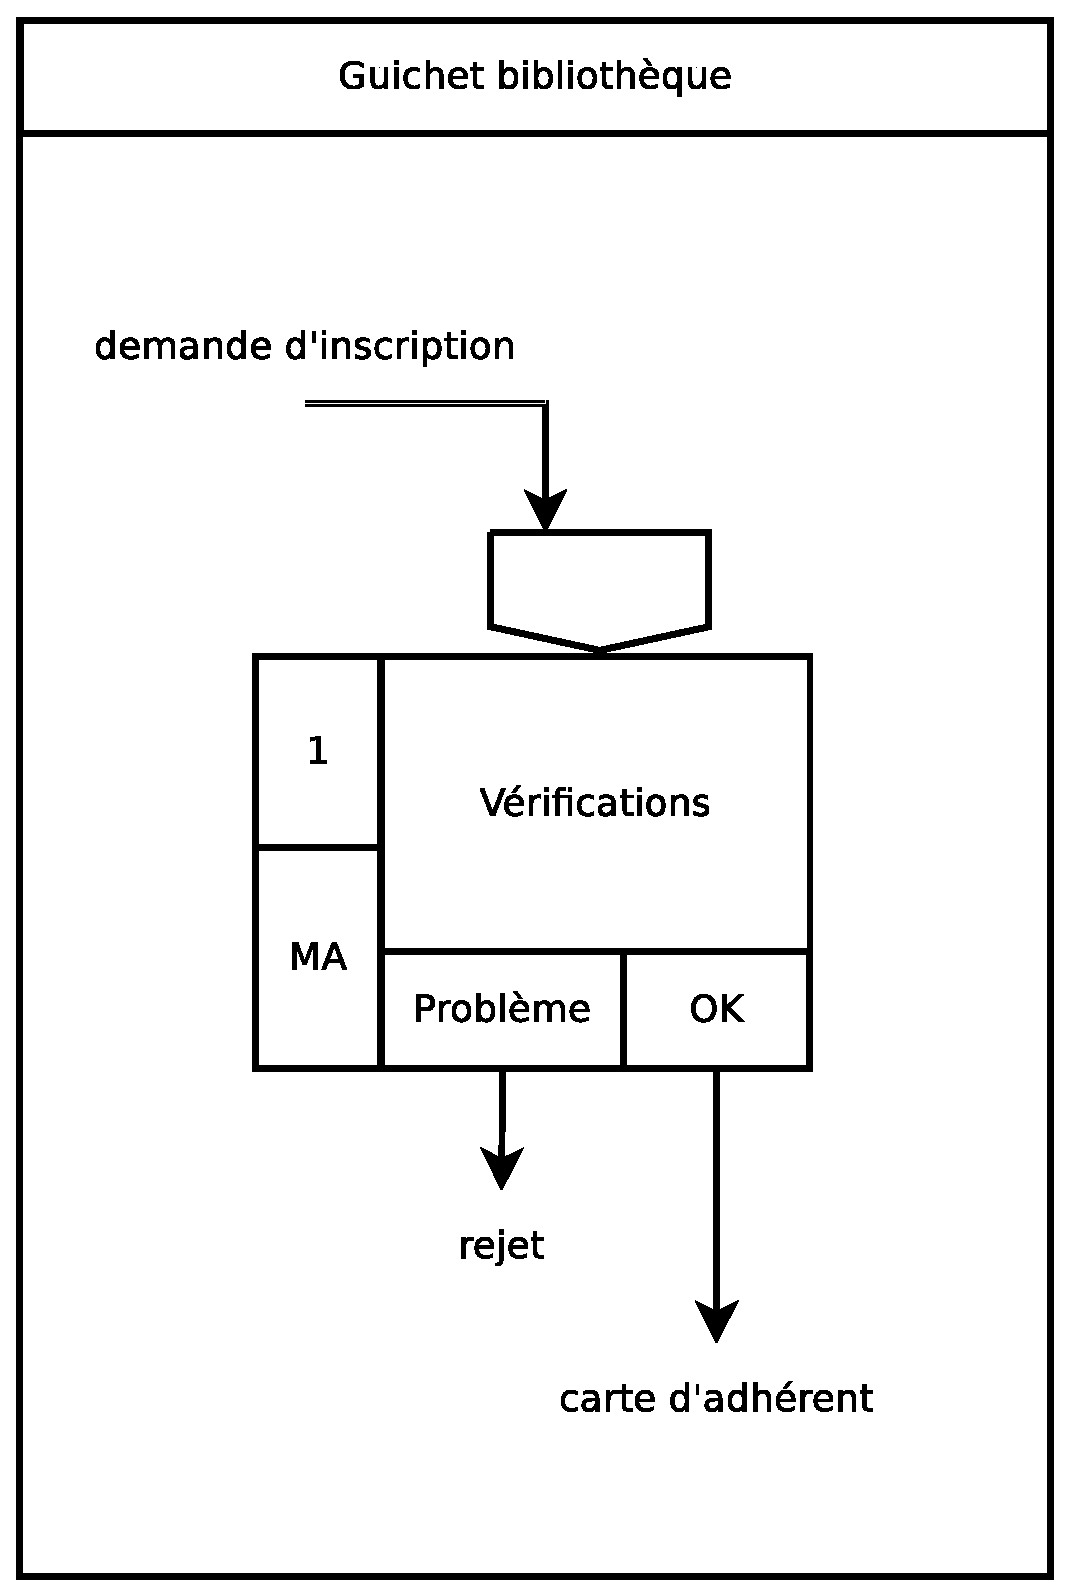
\includegraphics[height=5cm]{images/cc1_mot1.eps}
    %\caption{\label{cc1_mot1} Bureau d'homologation}
    \end{center}
\end{figure}

\begin{figure}[!htb]
    \begin{center}
    %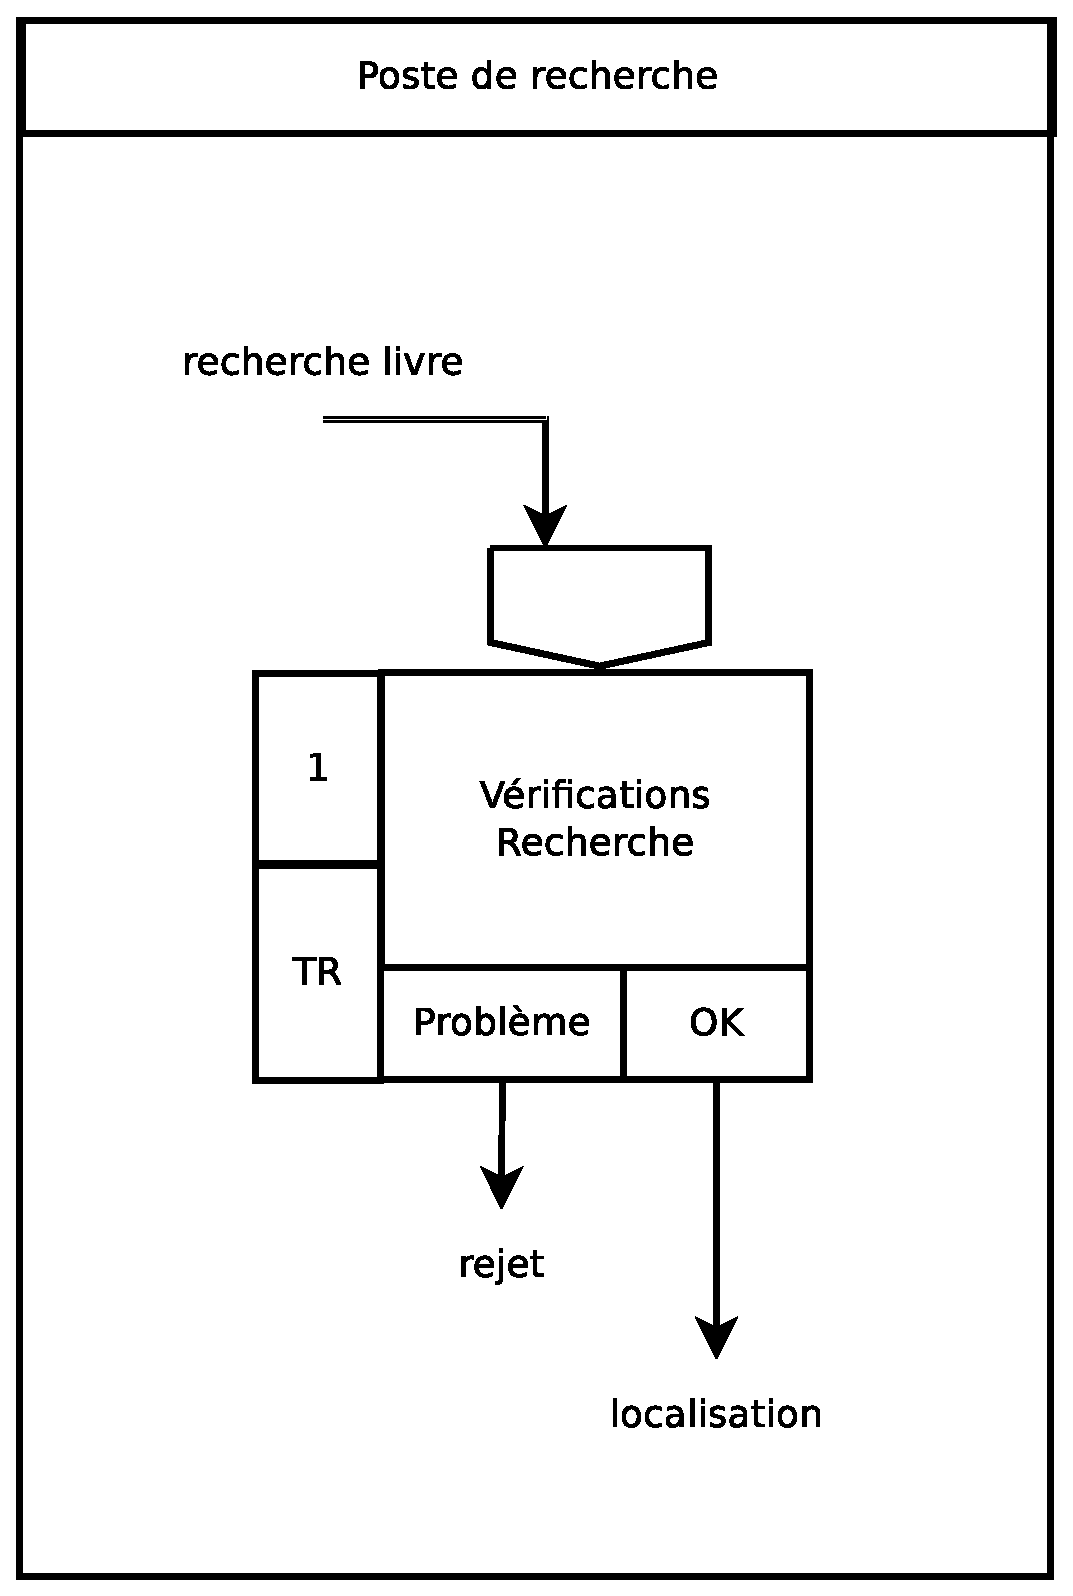
\includegraphics[height=8cm]{images/cc1_mot2.eps}
    %\caption{\label{cc1_mot2} Bureau du club et bureau de classement}
    \end{center}
\end{figure}


\newpage
\section*{Modèle Organisationel de Données}

On commence par déterminer les différents sites de notre système d'information :\\

\begin{figure}[!h]
\begin{tabular}{l l}
%
%
\end{tabular}
    \caption{\label{sites} Sites}
\end{figure}

\newpage
On détermine ensuite les droits d'accès pour les entités et les asssociations porteuses de données :\\

\begin{figure}[!htb]
\begin{tabular}{| l | c | c | c | c | c | c | c | c | c | c | c | c | c | c | c | c |}
%
   \hline
                  & \multicolumn{4}{| c |}{Sec. du club} & \multicolumn{4}{| c |}{Org. de compét.} & \multicolumn{4}{| c |}{Gest. des homolog.} & \multicolumn{4}{| c |}{Gest. du class.} \\
   \hline
                  & C & L & E & S & C & L & E & S & C & L & E & S & C & L & E & S \\
%
\end{tabular}
    \caption{\label{droits} Droits}
\end{figure}

\newpage
On en déduit les modèles d'organisations de données suivants : \\

\begin{figure}[!htb]
    \begin{center}
    %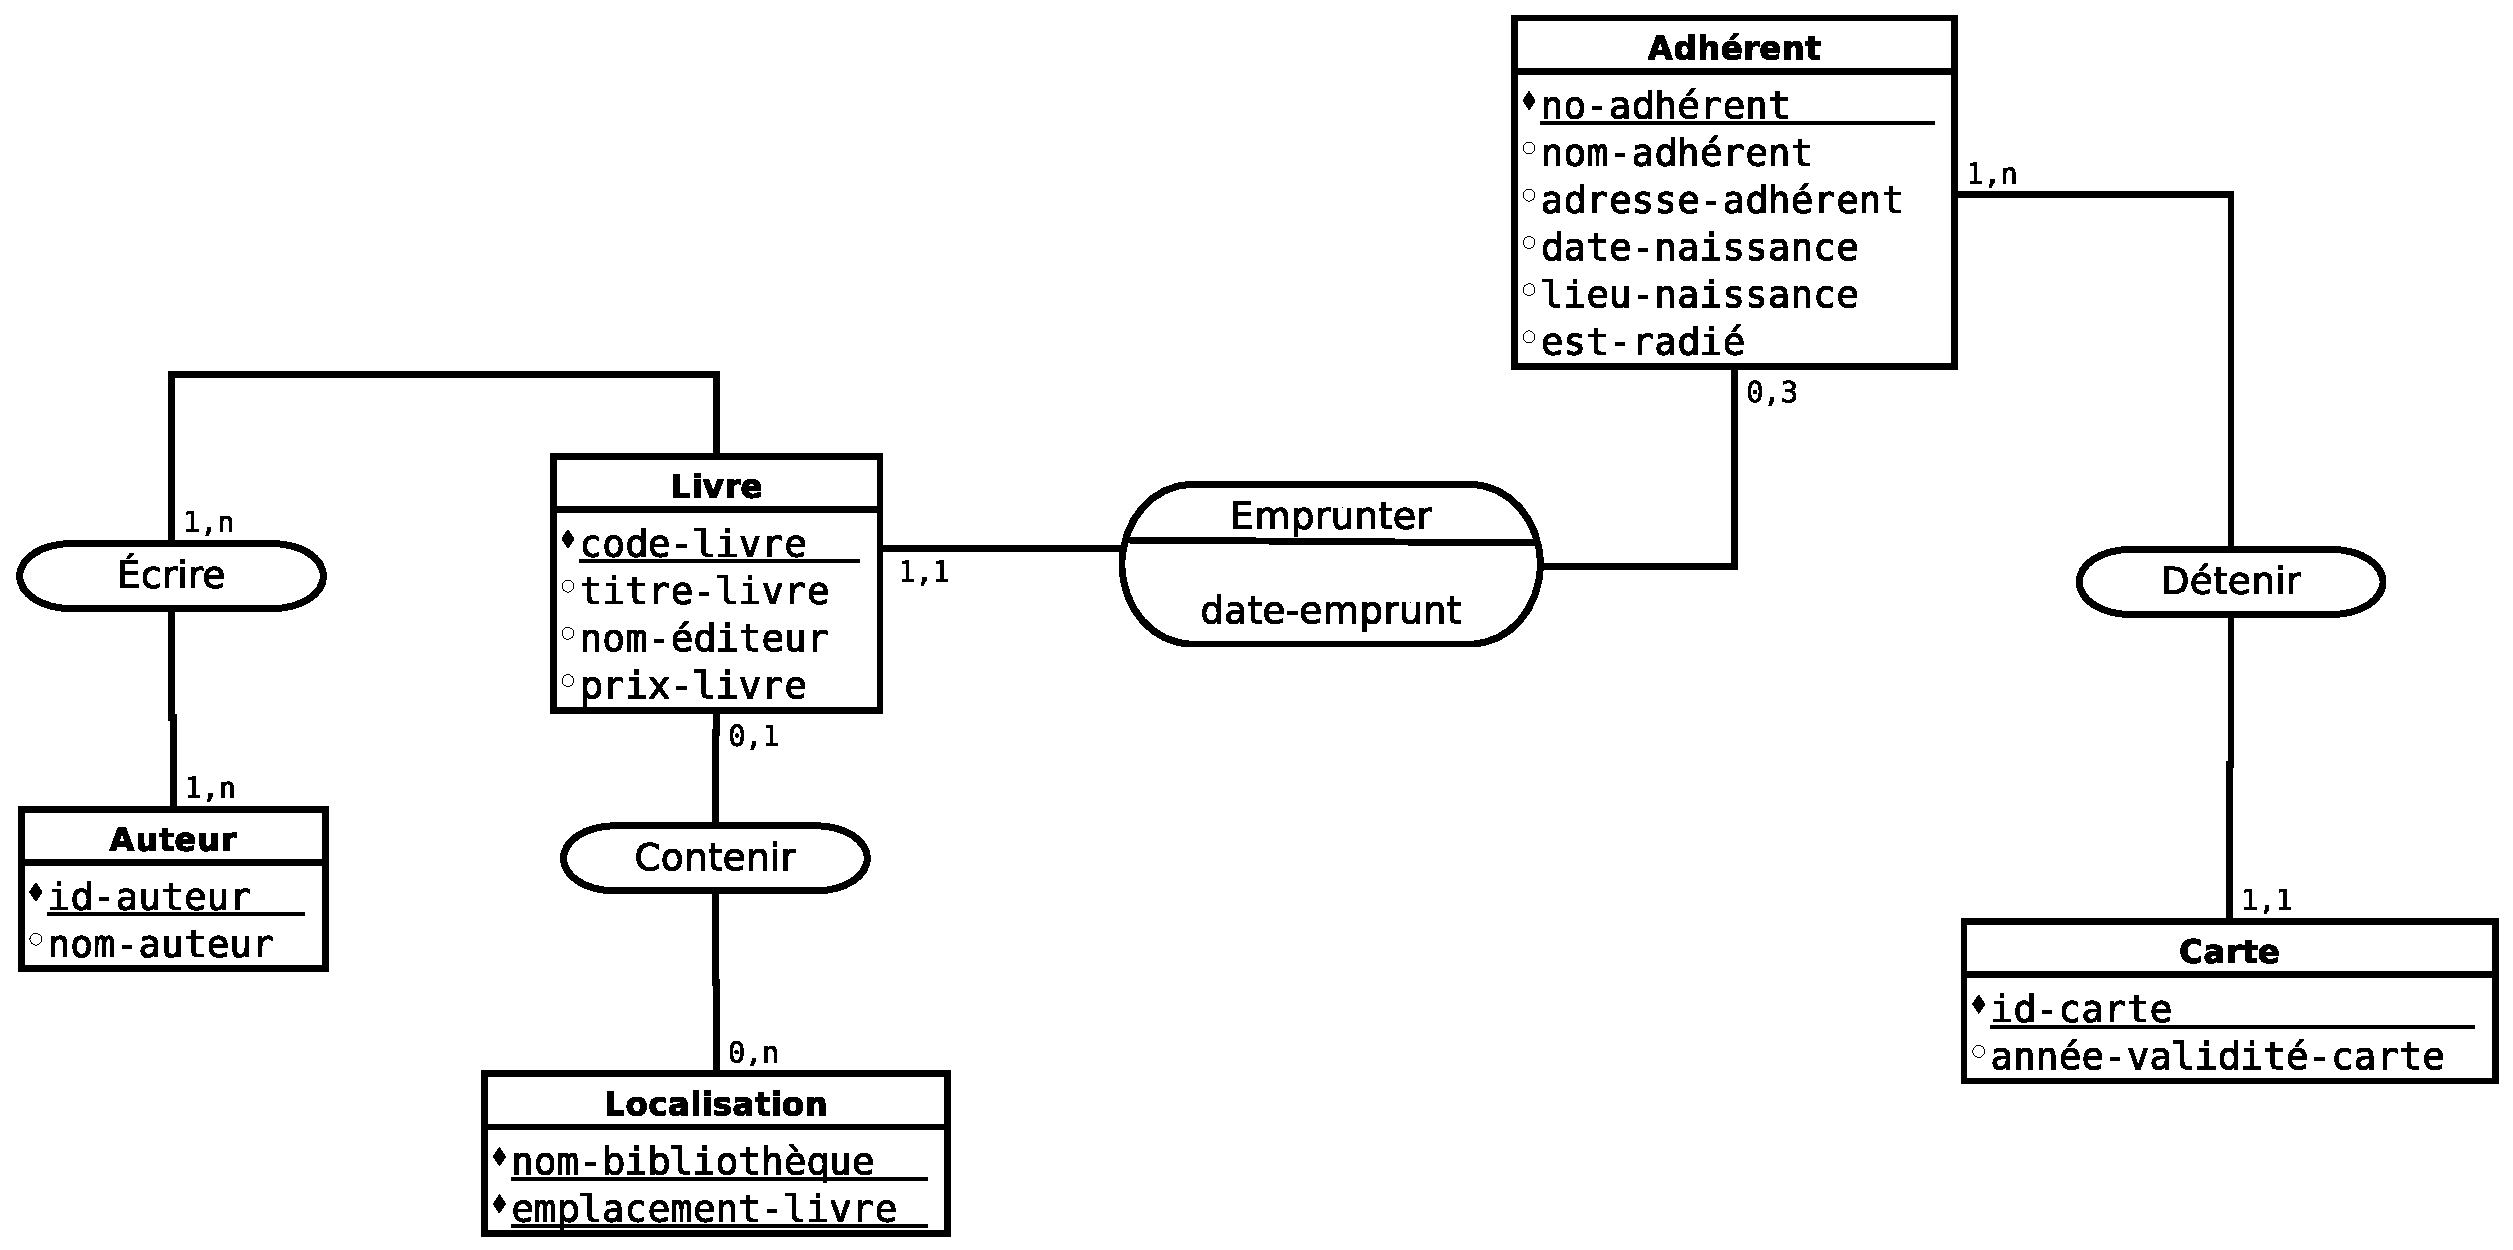
\includegraphics[width=11.5cm]{images/cc1_mod1.eps}
    \caption{\label{cc1_mod1} MOD Salle du club}
    \end{center}
\end{figure}

\begin{figure}[!htb]
    \begin{center}
    %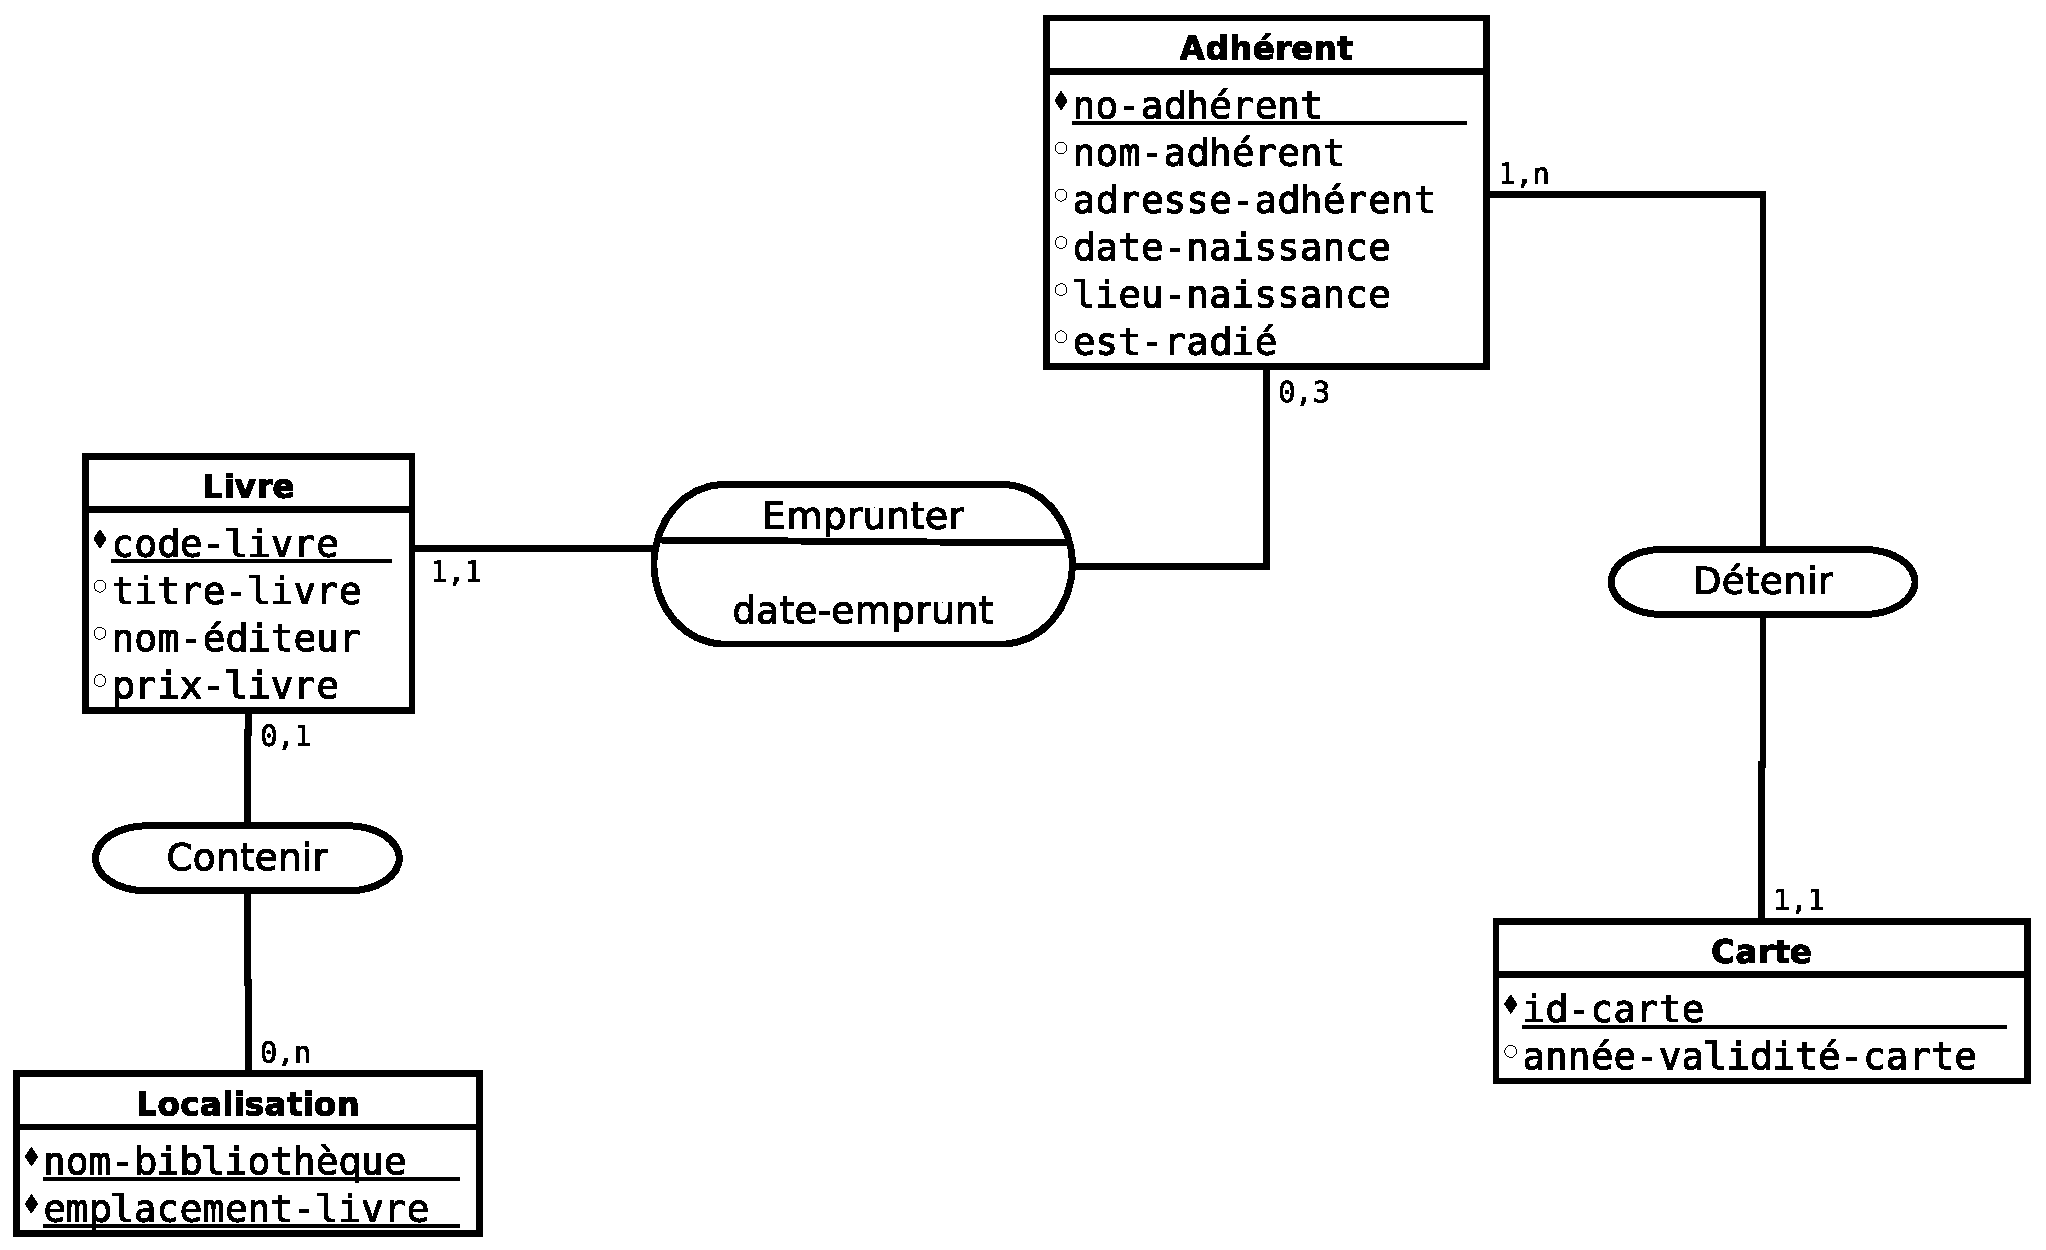
\includegraphics[width=11.5cm]{images/cc1_mod2.eps}
    \caption{\label{cc1_mod2} MOD Siège de la fédération}
    \end{center}
\end{figure}

